%%%%%%%%%%%%%%%%%%%%%%%%%%%%%%%%%%%%%%%%%%%%%%%%%%%%%%%%%%%%%%%%%%%%%%
% LaTeX Template: Beamer arrows
%
% Source: http://www.texample.net/
% Feel free to distribute this template, but please keep the
% referal to TeXample.net.
% Date: Nov 2006
% 
%%%%%%%%%%%%%%%%%%%%%%%%%%%%%%%%%%%%%%%%%%%%%%%%%%%%%%%%%%%%%%%%%%%%%%
% How to use writeLaTeX: 
%
% You edit the source code here on the left, and the preview on the
% right shows you the result within a few seconds.
%
% Bookmark this page and share the URL with your co-authors. They can
% edit at the same time!
%
% You can upload figures, bibliographies, custom classes and
% styles using the files menu.
%
% If you're new to LaTeX, the wikibook is a great place to start:
% http://en.wikibooks.org/wiki/LaTeX
%
%%%%%%%%%%%%%%%%%%%%%%%%%%%%%%%%%%%%%%%%%%%%%%%%%%%%%%%%%%%%%%%%%%%%%%

\documentclass{beamer} %
\usetheme{CambridgeUS}
\usepackage[latin1]{inputenc}
\usefonttheme{professionalfonts}
\usepackage[authoryear]{natbib}
\usepackage{times}
\usepackage{tikz}
\usepackage{amsmath}
\usepackage{verbatim}
\usetikzlibrary{arrows,shapes}
\usepackage[absolute,overlay]{textpos}
\usepackage{graphicx}

\setbeamercolor{framesource}{fg=gray}
\setbeamerfont{framesource}{size=\tiny}

\newcommand{\source}[1]{\begin{textblock*}{5cm}(7.7cm,8.6cm)
    \begin{beamercolorbox}[ht=0.5cm,right]{framesource}
        \usebeamerfont{framesource}\usebeamercolor[fg]{framesource} Source: {#1}
    \end{beamercolorbox}
\end{textblock*}}

\newcommand{\norm}[1]{\left\lVert#1\right\rVert}

\makeatother
\setbeamertemplate{footline}
{
  \leavevmode%
  \hbox{%
  \begin{beamercolorbox}[wd=.3\paperwidth,ht=2.25ex,dp=1ex,center]{author in head/foot}%
    \usebeamerfont{author in head/foot}\insertshortauthor
  \end{beamercolorbox}%
  \begin{beamercolorbox}[wd=.4\paperwidth,ht=2.25ex,dp=1ex,center]{title in head/foot}%
    \usebeamerfont{title in head/foot}\insertshorttitle\hspace*{3em}
  \end{beamercolorbox}
  \begin{beamercolorbox}[wd=.3\paperwidth,ht=2.25ex,dp=1ex,right]{date and frame number in head/foot}%
    \insertdate \quad \insertframenumber{} / \inserttotalframenumber\hspace*{1ex}
  \end{beamercolorbox}}%
  \vskip0pt%
}
\makeatletter
\setbeamertemplate{navigation symbols}{}

\author[Ditz, Hanssen, Sp\"{a}th]{Jonas Ditz, Friederike Hanssen, Julian Sp\"{a}th}
\title[TSS Prediction Workflow]{Integrated Workflow for Automated Transcription Start Site Prediction in Prokaryotes}
\institute{Data Management in Quantitative Biology\\ Dr. Sven Nahnsen\\ Sven Fillinger\\ University of T\"{u}bingen}

\begin{document}

\begin{comment}
:Title: Beamer arrows
:Tags: Remember picture, Beamer, Physics & chemistry, Overlays
:Use page: 3

With PGF/TikZ version 1.09 and later, it is possible to draw paths between nodes across
different pictures. This is a useful feature for presentations with the
Beamer package. In this example I've combined the new PGF/TikZ's overlay feature
with Beamer overlays. Download the PDF version to see the result.

**Note.** This only works with PDFTeX, and you have to run PDFTeX twice.

| Author: Kjell Magne Fauske

\end{comment}


% For every picture that defines or uses external nodes, you'll have to
% apply the 'remember picture' style. To avoid some typing, we'll apply
% the style to all pictures.
\tikzstyle{every picture}+=[remember picture]

% By default all math in TikZ nodes are set in inline mode. Change this to
% displaystyle so that we don't get small fractions.
\everymath{\displaystyle}

\begin{frame}
 \titlepage
\end{frame}

\begin{frame}{Overview}
 \tableofcontents
\end{frame}

\section{Introduction}

\begin{frame}{TSS Prediction}
 
\end{frame}

\begin{frame}{Technical Specs}
 
\end{frame}

\section{Workflow}
\begin{frame}{Overview}
 \tableofcontents[currentsection]
\end{frame}

\begin{frame}{Workflow Structure}
  \centering
  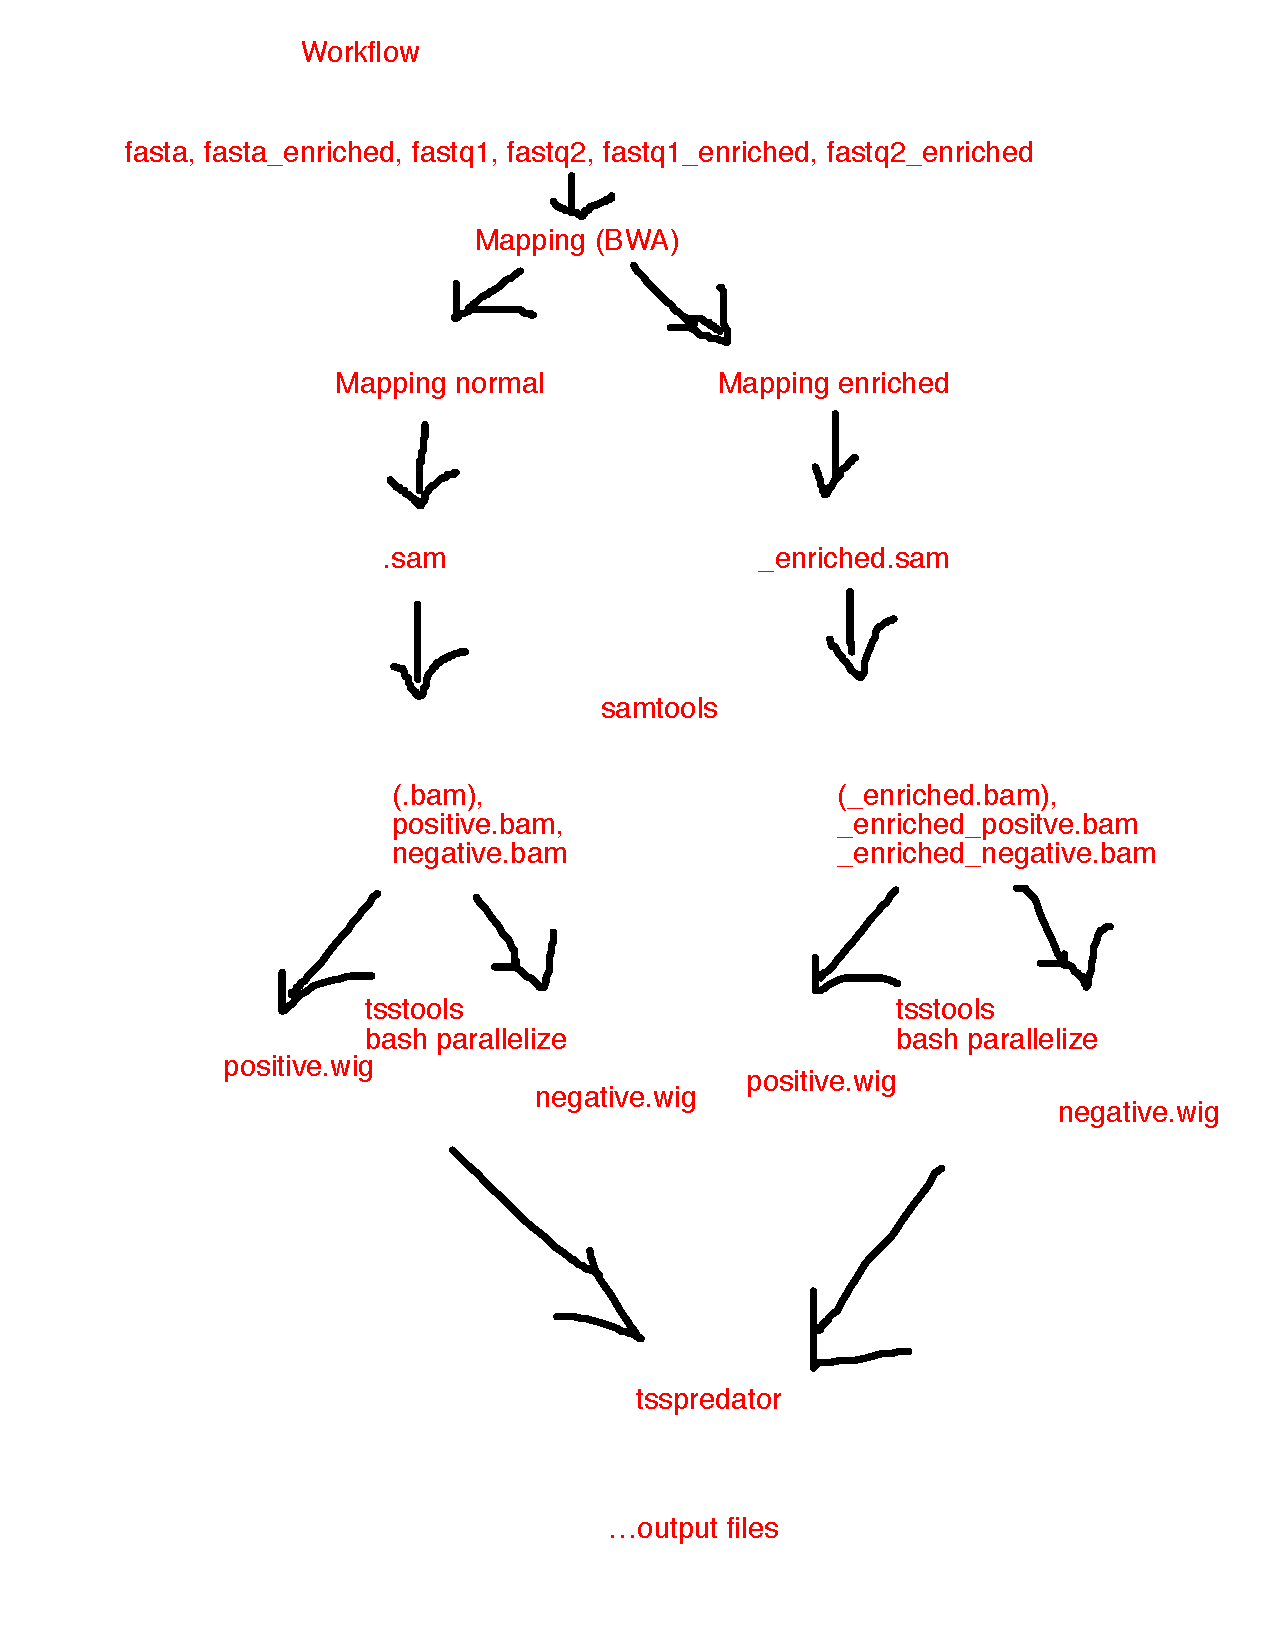
\includegraphics[width=0.5\textwidth]{../paper/workflow_sketch.pdf}
\end{frame}

\section{Outlook}
\begin{frame}{Overview}
 \tableofcontents[currentsection]
\end{frame}

\begin{frame}{Future Improvements}
 \begin{itemize}
  \item New Docker Modules
  \item Cloud Integration
  \item Fun, Fun, and more Fun
 \end{itemize}
\end{frame}

\begin{frame}[allowframebreaks]{References}
 \bibliographystyle{apalike}
 \bibliography{../paper/mylit.bib}
\end{frame}

% \begin{frame}
% \frametitle{Rigid body dynamics}
% 
% \tikzstyle{na} = [baseline=-.5ex]
% 
% \begin{itemize}[<+-| alert@+>]
%     \item Coriolis acceleration
%         \tikz[na] \node[coordinate] (n1) {};
% \end{itemize}
% 
% % Below we mix an ordinary equation with TikZ nodes. Note that we have to
% % adjust the baseline of the nodes to get proper alignment with the rest of
% % the equation.
% \begin{equation*}
% \vec{a}_p = \vec{a}_o+\frac{{}^bd^2}{dt^2}\vec{r} +
%         \tikz[baseline]{
%             \node[fill=blue!20,anchor=base] (t1)
%             {$ 2\vec{\omega}_{ib}\times\frac{{}^bd}{dt}\vec{r}$};
%         } +
%         \tikz[baseline]{
%             \node[fill=red!20, ellipse,anchor=base] (t2)
%             {$\vec{\alpha}_{ib}\times\vec{r}$};
%         } +
%         \tikz[baseline]{
%             \node[fill=green!20,anchor=base] (t3)
%             {$\vec{\omega}_{ib}\times(\vec{\omega}_{ib}\times\vec{r})$};
%         }
% \end{equation*}
% 
% \begin{itemize}[<+-| alert@+>]
%     \item Transversal acceleration
%         \tikz[na]\node [coordinate] (n2) {};
%     \item Centripetal acceleration
%         \tikz[na]\node [coordinate] (n3) {};
% \end{itemize}
% 
% % Now it's time to draw some edges between the global nodes. Note that we
% % have to apply the 'overlay' style.
% \begin{tikzpicture}[overlay]
%         \path[->]<1-> (n1) edge [bend left] (t1);
%         \path[->]<2-> (n2) edge [bend right] (t2);
%         \path[->]<3-> (n3) edge [out=0, in=-90] (t3);
% \end{tikzpicture}
% \end{frame}
\end{document}